\documentclass[french]{beamer}

%Erreur encoding?
\usepackage[T1]{fontenc}
% Animations
\usepackage{xmpmulti}
%Arbre pour goal babling
\usepackage{tikz}
\usetikzlibrary{trees}
%Centrer verticalement les tableaux
\usepackage{array}
\usepackage{changepage}
%Coloration des frames avec mathrice.sty
\usepackage{mathrice}
\usepackage{caption}
\usepackage{graphicx}
\graphicspath{{./graphics/}}
% Merge cellule verticalement tableau
\usepackage{multirow}
\usepackage{babel}

% Enlève les boutons de navigation des frames
\beamertemplatenavigationsymbolsempty

% Ajoute le logo FST sur chaque slides
\setbeamertemplate{background}{
    \begin{tikzpicture}[remember picture,overlay]
    \node[anchor=south west] at (current page.south west) {\includegraphics[height=1cm]{Logo_FST.jpg}};
\end{tikzpicture}}

% Numérotation des slides
\setbeamertemplate{footline}[frame number]

% Frame section dans un rectangle bleu foncé
\AtBeginSection[]{
  \begin{frame}
    \vfill
    \centering
    \begin{beamercolorbox}[sep=8pt,center,shadow=true,rounded=true]{title}
        \usebeamerfont{title}\insertsectionhead\par
    \end{beamercolorbox}
    \vfill
  \end{frame}
}

% Page de garde
\title{Comment découvrir son corps?}
\author{Lucas SCHWAB}
\date{Mars - Août 2019}

%%%%%%%%%%%%%%%%%%%%%%%%%%%%%%%%%%%%
%%%%%%%%%%%%% Document %%%%%%%%%%%%%
%%%%%%%%%%%%%%%%%%%%%%%%%%%%%%%%%%%%
\begin{document}

% Page de garde
\begin{frame}
    \begin{center}
        \begin{beamercolorbox}[sep=8pt,center]{title}
            \usebeamerfont{title}
            \Huge \textbf{Stage Master 2}

            \huge Comment découvrir son corps?
        \end{beamercolorbox}
        \vfill

        Lucas SCHWAB

        \vfill

        Encadrants:

        Amine BOUMAZA
        \&
        Alain DUTECH

        \vfill

        \begin{tabular}{m{0.4\textwidth} m{0.4\textwidth}}
            \includegraphics[height=50pt]{logo_loria_complet.jpg}
            &
            \'Equipe:
            LARSEN
        \end{tabular}
    \end{center}

\end{frame}

%-----------------------------------

% Sommaire
\begin{frame}
    \hfill
    \parbox[t]{.88\textwidth}{
        \begin{minipage}[c][0.75\textheight]{0.88\textwidth}
        \tableofcontents
        \end{minipage}
    }
    % Introduction
    %     Contexte
    %     Babling
    % Travail Realise
    %     Principe
    %     Algorithmes
    % Apprentissage
    %     Processus
    %     Resultats
    % Conclusion
\end{frame}

%###################################
\section{Introduction}

% Contexte
\begin{frame}
    \frametitle{Contexte}

    \begin{tikzpicture}[overlay]
        \node at (7,-2.5) {\includegraphics[width=.7\textwidth]{contexte.png}};
    \end{tikzpicture}

    But: Monde réel
    
    Robot: Commande

    \phantom{}

    Fonction: Monde Réel $\rightarrow$ Commande ?

    \vfill

\end{frame}

%-----------------------------------

% Comment calculer, cinématique inverse
\begin{frame}
    \frametitle{Cinématique Inverse}

    \large Exemple avec un bras robotique :

    \includegraphics[width=\textwidth]{Modelisation_Diagram_w_espaces_w_function.png}

    % Directe: on a besoin du modèle du robot pour calculer la position, il faut connaitre l'ordre et l'orientation des articulations.
    % Inverse: même en disposant du modèle, cette fonction reste difficile à calculer
\end{frame}

%-----------------------------------

%Présenter l'etat des choses
\begin{frame}
    \frametitle{Cinématique Inverse}

    \begin{tabular}{m{0.60\textwidth} m{0.4\textwidth}}
        \tikzstyle{every node}=[draw=black,thick,anchor=west]
        \tikzstyle{selected}=[draw=red,fill=red!30]
        \tikzstyle{optional}=[dashed,fill=gray!50]
        \begin{tikzpicture}[
            grow via three points={one child at (0.5,-0.7) and
            two children at (0.5,-0.7) and (0.5,-1.4)},
            edge from parent path={(\tikzparentnode.south) |- (\tikzchildnode.west)}]
                \node {Cinématique Inverse}
                child { node { Avec modèle } 
                    child { node { Solution Analytique } }
                    child { node { Optimisation } }
                    child { node { ... } }
                }
                child [missing] {}
                child [missing] {}
                child [missing] {}
                child { node { Sans modèle } 
                    child { node [selected] { Goal Babling} }
                    child { node { ... } }
                };
        \end{tikzpicture}

        &

        \footnotesize

        \phantom{}

        \vspace{3mm}

        Oudeyer et Kaplan (2007) \cite{OudeyerEtKaplan}
        
        \vspace{2mm}

        Baranes et Oudeyer (2010) \cite{GoalBabling}

        Rolf et al. (2011) \cite{rolfetautre}

        Jamone et al. (2011) \cite{jamone}

        % The idea of goal babbling was proposed by Oudeyer and Kaplan (2007) (p. 8). Computation implementations were then proposed by Baranes and Oudeyer (2010); Rolf et al. (2011) and Jamone et al. (2011). 

    \end{tabular}

    % Todo : REF
    % Liste des algo
    % moi c'est SANS modèle du robot
    % Je dois être aussi précis que d'autres
    % Je dois couvrir l'espace autant que les autres
\end{frame}

%-----------------------------------

% Mon travail -> Babling & Ergo
\begin{frame}
    \frametitle{Poppy Ergo Jr}
    
    \center
    \includegraphics[width=0.5\textwidth]{Poppy_Ergo_Jr.png}
    
\end{frame}

%-----------------------------------

% Babling: inspiration du processus développementale
\begin{frame}
    \frametitle{Goal Babling}

    \center
    \begin{tabular}[]{m{0.4\textwidth} m{0.5\textwidth}}
        \includegraphics[width=0.4\textwidth]{baby-walk.jpg}  
        
        &
        
        \center        Processus Développemental

        \vspace{5mm}

        {\large Nouveau Q $\rightarrow$ Nouveau X}

        \rotatebox[origin=c]{180}{$\Lsh$}
        Nouvelle expérience
    \end{tabular}

\end{frame}

%###################################
\section{Travail Réalisé}

% Expliquer la fonction f: X -> Q
\begin{frame}
    \frametitle{Cinématique Inverse}

    \center
    \begin{tabular}{m{0.4\textwidth} m{0.5\textwidth}}
        Fonction: 
        
        Monde réel $\rightarrow$ Commande

        \vspace{3mm}

        \center
        \Large
        F: 
        \large
        X $\rightarrow$ Q \nonumber

        \vspace{20mm}

        \phantom{}

        &

        \phantom{}

        \vspace{1mm}

        \center
        Expérience du robot

        \vspace{3mm}

        Catalogue

        \vspace{2mm}

        \begin{tabular}{||c | c ||}
            \hline
            Observation (X) & Commande (Q) \\
            \hline
            x1, y1, z1 & $\theta_{a1}, \theta_{b1}, ...$\\
            x2, y2, z2 & $\theta_{a2}, \theta_{b2}, ...$\\
            x3, y3, z3 & $\theta_{a3}, \theta_{b3}, ...$\\
            ... & ...\\
            \hline
        \end{tabular}
    \end{tabular}

\end{frame}

%-----------------------------------

% Comment construire F
\begin{frame}
    \frametitle{Comment construire F ?}
    \center
    \tikzstyle{every node}=[draw=black,thick,anchor=west]
    \tikzstyle{selected}=[draw=red,fill=red!30]
    \tikzstyle{optional}=[dashed,fill=gray!50]
    \begin{tikzpicture}[
        grow via three points={one child at (0.5,-0.7) and
        two children at (0.5,-0.7) and (0.5,-1.4)},
        edge from parent path={(\tikzparentnode.south) |- (\tikzchildnode.west)}]
            \node {Cinématique Inverse}
            child { node { Sans modèle }
                child { node [selected] {Goal Babling} }
                child { node { ... } }
            }
            child [missing] {}
            child [missing] {}
            child { node [optional] { Avec Modèle }
                child { node [optional] { Solution Analytique } }
                child { node [optional] { Optimisation } }
                child { node [optional] { ... } }
            };
    \end{tikzpicture}

\end{frame}

%-----------------------------------

% Expliquer Goal Babling
\begin{frame}
    \frametitle{Goal Babling}

    \begin{tabular}{m{0.4\textwidth} m{0.5\textwidth}}

        {\center Perturbation d'une posture}

        \includegraphics[width=0.4\textwidth]{randomize_posture.png}

        \vspace{15mm}

        \phantom{}

        &

        \center
        \underline{Suivre un but}
        
        \vspace{15mm}

        {\hspace{5mm} Utilisation du Catalogue}

        \begin{tabular}{||c | c ||}
            \hline
            Observation (X) & Commande (Q) \\
            \hline
            x1, y1, z1 & $\theta_{a1}, \theta_{b1}, ...$\\
            x2, y2, z2 & $\theta_{a2}, \theta_{b2}, ...$\\
            x3, y3, z3 & $\theta_{a3}, \theta_{b3}, ...$\\
            ... & ...\\
            \hline
        \end{tabular}
        
    \end{tabular}

\end{frame}

%-----------------------------------

% Motor Babling
\begin{frame}
    \frametitle{Motor Babling}

    \begin{tabular}{m{.35\textwidth} m{.55\textwidth}}
        
        % \center
        Commande Aléatoire

        \includegraphics[width=.30\textwidth]{poppy_motor_babling/frame-2.png}

        &

        \Large
        \underline{Initialisation du catalogue}

        \vspace{10mm}

        \normalsize
        \center
        Distribution des observations

        \includegraphics[width=.35\textwidth]{motor_babling_distribution.png}


    \end{tabular}

\end{frame}

%-----------------------------------

%Agnostic introduction
\begin{frame}
    \vfill
    \centering
    \begin{beamercolorbox}[sep=8pt,center,shadow=true,rounded=true]{title}
        \usebeamerfont{title}Agnostic Goal Generator\par
    \end{beamercolorbox}
    \vfill
\end{frame}

%-----------------------------------

% Goal Babling: Agnostique
\begin{frame}
    \frametitle{Agnostic Goal Generator}

    \center
    \multiinclude[<+>][format=png, graphics={width=.7\textwidth}]{agnostic_gg/frame}

\end{frame}

%-----------------------------------

%Frontier introduction
\begin{frame}
    \vfill
    \centering
    \begin{beamercolorbox}[sep=8pt,center,shadow=true,rounded=true]{title}
        \usebeamerfont{title}Algorithme Frontier\par
    \end{beamercolorbox}
    \vfill
\end{frame}

%-----------------------------------

% Goal babling: Frontier
\begin{frame}
    \frametitle{Goals on Grid \& Frontier}

    \center
    \multiinclude[<+>][format=png, graphics={width=.7\textwidth}]{frontier/frame}

    % La grille etc, chercher la frontière
\end{frame}



%###################################
\section{Expérimentation}

% Experience - lancer - mesurer
\begin{frame}
    \frametitle{Expérience}

    Choisir paramètres $\Rightarrow$ Lancer apprentissage $\Rightarrow$ Mesurer résultat

    % Je possède 3 variantes de babling, qui possèdent chacun plusieurs paramètres.
    % Comme tous utilisent de l'aléatoire pendant l'apprentissage, j'exécute plusieurs expériences afin d'avoir une distribution à analyser comme résultat

    \vfill

    \center
    \tikzstyle{every node}=[draw=black,thick,anchor=west]
    \tikzstyle{selected}=[draw=red,fill=red!30]
    \tikzstyle{optional}=[dashed,fill=gray!50]
    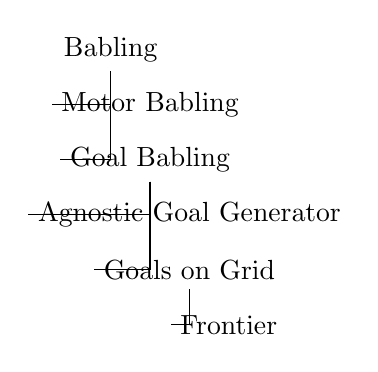
\begin{tikzpicture}[
        grow via three points={one child at (0.5,-0.7) and
        two children at (0.5,-0.7) and (0.5,-1.4)},
        edge from parent path={(\tikzparentnode.south) |- (\tikzchildnode.west)}]
            \node {Babling}
            child { node { Motor Babling } }
            child { node { Goal Babling }
                child { node {Agnostic Goal Generator} }
                child { node {Goals on Grid} 
                    child { node {Frontier} }
                }
            };
    \end{tikzpicture}

    % Présenter les paramètres, introduire couverture et précision

\end{frame}

%-----------------------------------

\begin{frame}
    \frametitle{Couverture: Volume et Remplissage}
    
    \begin{tabular}{c c}
        \includegraphics[width=.45\textwidth]{couverture/volu-1.png}

        &

        \includegraphics[width=.45\textwidth]{couverture/remp-1.png}

        \\

        Enveloppe Convexe

        &

        Cellules visitées

    \end{tabular}

\end{frame}

%-----------------------------------

\begin{frame}
    \frametitle{Précision: Erreur sur une liste de test}
    
    \huge$\sum\limits_{g \in goals} \frac{ d( g, G(  F(  g  )  ) )}
    {nb\_goals}$
    
    \vfill
    \center \normalsize
    Représentation de la liste des buts:

    \raggedleft
    \begin{tabular}{c c}
        \includegraphics[width=.35\textwidth]{goal_list_front_2.png} &
        \includegraphics[width=.35\textwidth]{goal_list_top_2.png}
        \\
        Vue de face & Vue du dessus
    \end{tabular}
\end{frame}

%-----------------------------------

% Resultats Motor Babling
\begin{frame}
    \frametitle{Résultats: Motor Babling}

    Paramètre $p$ analysé: Nombre d'entrée dans le catalogue
    \vfill

    \begin{tabular}{c c}
        Couverture (volume) & Précision (distance liste ikpy)
        \\
        \includegraphics[width = 0.45\textwidth]{1mb_1k-100kstep_couver.png} &
        \includegraphics[width = 0.45\textwidth]{1mb_1k-100kstep_moy_ik.png}
        \\
        $p \nearrow$ = Couverture \color{green}$\nearrow$
        &
        $p \nearrow$ = Précision \color{green}$\nearrow$
    \end{tabular}
\end{frame}

%-----------------------------------

% Resultats Goal Babling
\begin{frame}
    \frametitle{Résultats: Goal Babling}

    Paramètre $p$ analysé: Proportion de Motor Babling à l'initialisation
    \vfill
    
    \begin{tabular}{c c}
        Couverture (volume) & Précision (distance liste ikpy)
        \\
        \includegraphics[width = 0.45\textwidth]{0.2-.01mb_couver.png} &
        \includegraphics[width = 0.45\textwidth]{0.2-.01mb_moy_ik.png}
        \\
        $p \nearrow$ = Variance Couverture \color{green}$\searrow$
        &
        $p \nearrow$ = Variance Précision \color{orange}$\nearrow$
    \end{tabular}
\end{frame}

%-----------------------------------

% Résultats Agnostique
\begin{frame}
    \frametitle{Résultats: Agnostic Goal Generator}

    Paramètre $p$ analysé: Taux d'extension de la zone des buts
    \vfill
    
    \begin{tabular}{c c}
        Couverture (volume) & Précision (distance liste ikpy)
        \\
        \includegraphics[width = 0.45\textwidth]{Agn_.7-1.4exp_couver.png} &
        \includegraphics[width = 0.45\textwidth]{Agn_.7-1.4exp_moy_ik.png}
        \\
        $p \nearrow$ = Couverture \color{green}$\nearrow$
        &
        $p \nearrow$ = Précision \color{orange}$\searrow$
    \end{tabular}
\end{frame}

%-----------------------------------

% Résultats Frontier
\begin{frame}
    \frametitle{Résultats: Frontier}

    Paramètre $p$ analysé: Probabilité d'exploration
    \vfill
    
    \begin{tabular}{c c}
        Couverture (volume) & Précision (distance liste ikpy)
        \\
        \includegraphics[width = 0.45\textwidth]{Fro_.01-.5-.9pexp_couver.png} &
        \includegraphics[width = 0.45\textwidth]{Fro_.01-.5-.9pexp_moy_gl.png}
        \\
        $p \nearrow$ = Couverture $\rightarrow$
        &
        $p \nearrow$ = Précision $\rightarrow$
    \end{tabular}
\end{frame}

%-----------------------------------

% Comparer les 3 algorithmes
\begin{frame}
    \frametitle{Résultats}

    Comparaison des 3 algorithmes
    \vfill

    \begin{tabular}{c c}
        Couverture (volume) & Précision (distance liste but)
        \\
        \includegraphics[width = 0.45\textwidth]{ALL_couver.png} &
        \includegraphics[width = 0.45\textwidth]{ALL_moy_gl.png}
    \end{tabular}
\end{frame}

%###################################
\section{Conclusion}

% Conclusion
\begin{frame}

    \begin{itemize}
        \item Cinématique Inverse pour Poppy Ergo Jr
        \item Babling
        \begin{itemize}
            \item Motor Babling
            \item Agnostic Goal Generator
            \item Frontier
        \end{itemize}
        \item Résultats
        \begin{itemize}
            \item Contraintes ignorées
            \item Incompatibilité Poppy Ergo Jr
            \item Meilleur que Motor Babling: aléatoire total
        \end{itemize}
    \end{itemize}
\end{frame}

%-----------------------------------

\begin{frame}
    \center
    \Huge Merci de votre attention
    
    Avez-vous des questions ?
\end{frame}

%-----------------------------------

\begin{frame}
    \footnotesize
    \bibliographystyle{unsrt}
    \bibliography{sample}
\end{frame}

\end{document}